\documentclass[]{rptuseminar}

% Specify that the source file has UTF8 encoding
\usepackage[utf8]{inputenc}
% Set up the document font; font encoding (here T1) has to fit the used font.
\usepackage[T1]{fontenc}
\usepackage{lmodern}

% Load language spec
\usepackage[american]{babel}
% German article --> ngerman (n for »neue deutsche Rechtschreibung«)
% British English --> english

% Ffor bibliography and \cite
\usepackage{cite}

% AMS extensions for math typesetting
\usepackage[intlimits]{mathtools}
\usepackage{amssymb}
% ... there are many more ...


% Load \todo command for notes
\usepackage{todonotes}
% Sebastian's favorite command for large inline todonotes
% Caveat: does not work well with \listoftodos
\newcommand\todoin[2][]{\todo[inline, caption={2do}, #1]{
		\begin{minipage}{\linewidth-1em}\noindent\relax#2\end{minipage}}}

% Load \includegraphics command for including pictures (pdf or png highly recommended)
\usepackage{graphicx}

% Typeset source/pseudo code
\usepackage{listings}

% Load TikZ library for creating graphics
% Using the PGF/TikZ manual and/or tex.stackexchange.com is highly adviced.
\usepackage{tikz}
% Load tikz libraries needed below (see the manual for a full list)
\usetikzlibrary{automata,positioning}

% Load \url command for easier hyperlinks without special link text
\usepackage{url}

% Load support for links in pdfs
\usepackage{hyperref}

% Defines default styling for code listings
% \definecolor{pink}{rgb}{}
\definecolor{green_ulises}{rgb}{0.2,0.75,0}
\lstdefinelanguage{smtlib2} {
  morekeywords={set-logic, declare-const, assert, check-sat, get-model},
  sensitive=true,
  morecomment=[l]{;},
  morestring=[b]"
}

\lstset{%
  columns=flexible,
  keepspaces=true,
  tabsize=3,
  basicstyle={\fontfamily{tx}\ttfamily\small},
  stringstyle=\color{green_ulises},
  commentstyle=\color{black!80}
  identifierstyle=\slshape{},
  keywordstyle=\bfseries,
  numberstyle=\small\color{pink},
  backgroundcolor=\color{gray!5},
  numberblanklines=false,
  inputencoding={utf8},
  showstringspaces=false,
  belowskip=-1mm,
  escapeinside={//*}{\^^M} % Allow to set labels and the like in comments
}

% Defines a custom environment for indented shell commands
\newenvironment{displayshellcommand}{%
	\begin{quote}%
	\ttfamily%
}{%
	\end{quote}%
}

%%%%%%%%%%%%%%%%
\lstnewenvironment{haskell}{
  \vspace{1em}%
  \lstset{
    language=Haskell,
    columns=flexible,
    keepspaces=true,
    tabsize=3,
    basicstyle={\fontfamily{tx}\ttfamily\small},
    stringstyle=\color{green_ulises},
    commentstyle=\color{black!80},
    identifierstyle=\slshape{},
    keywordstyle=\bfseries,
    numberstyle=\small\color{pink},
    backgroundcolor=\color{gray!5},
    numberblanklines=false,
    inputencoding={utf8},
    belowskip=-1mm,
    escapeinside={//*}{\^^M} % Allow to set labels and the like in comments
  }
}{
  \vspace{1em}
}%%%%%%%%%%%%%%%%%%%%%%%%%%%%%%%%%%%%%%%%%%%%%%%%%%%%%%%%%%%%%%%

\title{Liquid Haskell}
\event{Seminar: Programming Languages in Winter term 2024/2025}
\author{Mehran Shahidi, Saba Safarnezhad
  \institute{Rheinland-Pfälzische Technische Universität Kaiserslautern-Landau, Department of Computer Science}}

%%%%%%%%%%%%%%%%%%%%%%%%%%%%%%%%%%%%%%%%%%%%%%%%%%%%%%%%%%%%%%%%%%%%%%%%%%%%%%%
\begin{document}
%%%%%%%%%%%%%%%%%%%%%%%%%%%%%%%%%%%%%%%%%%%%%%%%%%%%%%%%%%%%%%%%%%%%%%%%%%%%%%%

\maketitle

%%%%%%%%%%%%%%%%%%%%%%%%%%%%%%%%%%%%%%%%%%%%%%%%%%%%%%%%%%%%%%%%%%%%%%%%%%%%%%%

\begin{abstract}
  This report gives a brief overview of \textsc{LiquidHaskell}, a tool that extends Haskell with refinement types. 
  Refinement types are types that extends expressiveness of Haskell types systems by providing predicates that can verify
  invarients of the program. This report explains briefly how SMT solvers leveraged by \textsc{LiquidHaskell} and 
  how to use \textsc{LiquidHaskell} by providing some examples. Finally, we discuss the limitations of \textsc{LiquidHaskell} and compare it with other tools.
\end{abstract}

%%%%%%%%%%%%%%%%%%%%%%%%%%%%%%%%%%%%%%%%%%%%%%%%%%%%%%%%%%%%%%%%%%%%%%%%%%%%%%

\section{Introduction}
\label{sec:introduction}
Programming verfication is an important step in software developments. It is the process of
verifying that a program behaves as it expected. There has been a lot of research in this 
area and many tools have been developed. 
Type safety is one of the important features of programming languages that helps to prevent runtime errors.
Despite catching many errors at compile time, type systems are not powerful enough to catch all the errors.
On the other, testing is another way to verify the program, but it is not always possible to test all the possible inputs.
Consider the following example:

\begin{haskell}
  average    :: [Int] -> Int
  average xs = sum xs `div` length xs
\end{haskell}

The example above is a simple function that calculates the average of a list of integers. This can be a source of runtime
error if the list is empty. While this can be caught by testing, it is not always possible to test all the possible inputs.
Another way to verify the program is to use program verification tools. These tools use mathematical logic to check the program.
One of such tools that is used in Haskell programming language is \textsc{LiquidHaskell}. \textsc{LiquidHaskell} 
(LH) extends Haskell with refinement types which are types that extend the expressiveness of Haskell.
With refinement types, we can provide invariant that the program should satisfy. 

In this report, after a short backgrouund on program verfication using SMT in section \ref{sec:background}, we will explain 
how LH works and how it uses SMT solvers to 
verify the program in section \ref{sec:lh}. Then in section \ref{sec:example} we will provide some examples how to use 
LH to verify persistent stack. Finally in section \ref{sec:conclusions} we 
discuss the limiations of LH and compare it with other tools.

% E.~g.~ 
% ``quoting'' is done by using two backticks and two single quotes

\section{Background}
\label{sec:background}
\begin{description}
  \item[Refinement Types] Refinement types add predicates to the types \cite{jhala_programming_2020}. For example, consider the following type:


    \begin{haskell}
      {-@ incr :: Pos -> Pos @-}
      incr :: Int -> Int
      incr x = x + 1
    \end{haskell}

  \item[Predicate] Predicates are haskell expressions that evaluate to boolean.
  \item[SMT Solvers] SMT solvers are used to check the satisfiability of the predicates. 
  
\end{description}
\subsection{SMT Solvers}
SMT (Satisfiability Modulo Theories) solvers are tools that can check the satisfiability of logical formulas in a specific theory.
SMT solvers extends the concept of SAT solvers by adding theories (e.g., the theory of equality, 
of integer numbers, of real numbers, of arrays, of lists, and so on) to the boolean logic \cite{clarke_satisfiability_2018}.
While SAT solvers can only check the satisfiability of boolean formulas, SMT solvers can check the satisfiability of formulas 
that contain variables from different theories. 
As an example, consider the following formula:

\begin{equation}
  \varphi = (x \lor y) \land (\lnot x \lor z)
\end{equation}

SAT solver can check the satisfiability of the formula \(\varphi\) by checking if there is an assignment for the variables \(x, y, z\).
For instance, \(x = true, y = false, z = true\) is an assignment that makes \(\varphi\) \(true\). 

On the other hand, SMT solvers can check the satisfiability of formulas that contain variables that required arithmetic theory as following formula:
Figure \ref{fig:scholar}

\begin{equation}
  x + y \leq 10 \quad and \quad x = y - 7
\end{equation}

\subsection{Z3 SMT Solvers}
\subsubsection*{Overall System Architecture of Z3}

The overall system architecture of Z3 is designed to efficiently solve Satisfiability Modulo Theories (SMT) problems.
 Here's a detailed breakdown of the key components and their interactions:

\subsubsection{Interfaces to Z3}
Z3 can be interacted with using SMT-LIB2 scripts supplied as text files or through a pipe. Additionally,
high-level programming languages can make API calls to Z3, which are proxies for calls over a C-based API.
The tutorial focuses on using the Python front-end for interfacing with Z3.

\subsubsection{Logical Formulas}
Z3 accepts logical formulas built from atomic variables and logical connectives, which can include symbols defined by various theories.
These formulas use basic building blocks like Boolean variables, integers, and reals, combined with logical operators such as
\texttt{And}, \texttt{Or}, \texttt{Not}, \texttt{Implies}, and \texttt{Xor}. Z3 handles complex logical expressions by
integrating symbols from multiple theories, such as arrays and arithmetic, allowing it to model a wide range of problems.
The formulas generally follow the SMT-LIB2 standard, ensuring interoperability between different SMT solvers. 
This versatility makes Z3 a powerful tool for solving diverse logical problems efficiently.

\subsubsection{Theories}
Z3 supports multiple theories, including Equality and Uninterpreted Functions (EUF), Arithmetic (both linear and non-linear),
Arrays, Bit-Vectors, Algebraic Datatypes, Sequences, and Strings. Each theory has specialized decision procedures for solving
related formulas.

\subsubsection{Solver}
Z3 provides services for deciding the satisfiability of formulas. This includes handling incrementality, scopes, assumptions, 
cores, models, and other methods like statistics, proofs, and retrieving solver state. Specialized solvers are included for 
different types of problems

\subsubsection*{SMT Solver}
The SMT solver in Z3 is a general-purpose solver that integrates various theories to decide the satisfiability of logical formulas. 
It uses the CDCL(T) architecture, which combines Conflict-Driven Clause Learning (CDCL) with theory solvers.

\subsubsection*{Fixedpoint Solver}
The Fixedpoint solver in Z3 is used for reasoning about recursive definitions and fixed-point computations. 
It includes a Datalog engine and supports relational algebra and Property Directed Reachability (PDR) algorithms.

\subsubsection*{NLSat Solver}
The NLSat solver is specialized for non-linear arithmetic problems. 
It uses a combination of algebraic methods and SAT solving techniques to handle polynomial constraints.

\subsubsection*{SAT Solver}
The SAT solver in Z3 is designed for propositional logic problems. It uses advanced techniques like in-processing 
and co-processing to efficiently solve Boolean satisfiability problems.

\subsubsection*{QSAT Solver}
The QSAT solver handles quantified Boolean formulas (QBF). It extends the capabilities of the SAT solver to deal with quantifiers, 
providing solutions for more complex logical problems.


\subsubsection{Tactics}
Tactics in Z3 are used for pre-processing, simplifying formulas, and creating sub-goals. 
They are essential for breaking down complex problems into more manageable parts.

\subsubsection*{Preprocessing}
Preprocessing tactics simplify the input formulas before they are passed to the main solver. This can include techniques 
like constant propagation, simplification of arithmetic expressions, and elimination of redundant constraints.

\subsubsection*{Cube and Conquer}
The Cube and Conquer tactic is used to partition the search space into smaller sub-problems (cubes) that can be solved independently. 
This approach is particularly useful for parallel solving and can significantly reduce the overall solving time.

\subsubsection*{tacticals}
Tacticals are combinators that allow the composition of multiple tactics. Examples include:

\begin{itemize}
    \item \texttt{then}: Applies a sequence of tactics to the input goal.
    \item \texttt{par-then}: Applies tactics in parallel to the input goal.
    \item \texttt{or-else}: Applies the first tactic and, if it fails, applies the second tactic.
    \item \texttt{repeat}: Repeatedly applies a tactic until no subgoal is modified.
\end{itemize}

The architecture of Z3 is designed to be flexible and powerful, supporting a wide range of logical theories and providing
 robust solver services. It allows for efficient interaction through various interfaces and includes advanced features for
  optimization and logical analysis.

\subsubsection{Optimization}
Z3 provides optimization services that allow users to solve satisfiability problems while maximizing or minimizing objective functions. 
This is useful for problems that require finding the best solution under given constraints.

\subsubsection{Advanced Features}
Z3 includes specialized procedures for enumerating consequences (backbone literals), which are useful for certain types of logical analysis.


The architecture of Z3 is designed to be flexible and powerful, 
supporting a wide range of logical theories and providing robust solver services. It allows for efficient interaction through 
various interfaces and includes advanced features for optimization and logical analysis.

This LaTeX code will format the text with a section heading, a list of examples, and a concluding paragraph, making it clear 
and well-structured.


\begin{figure}[ht]
  \begin{center}
    \fbox{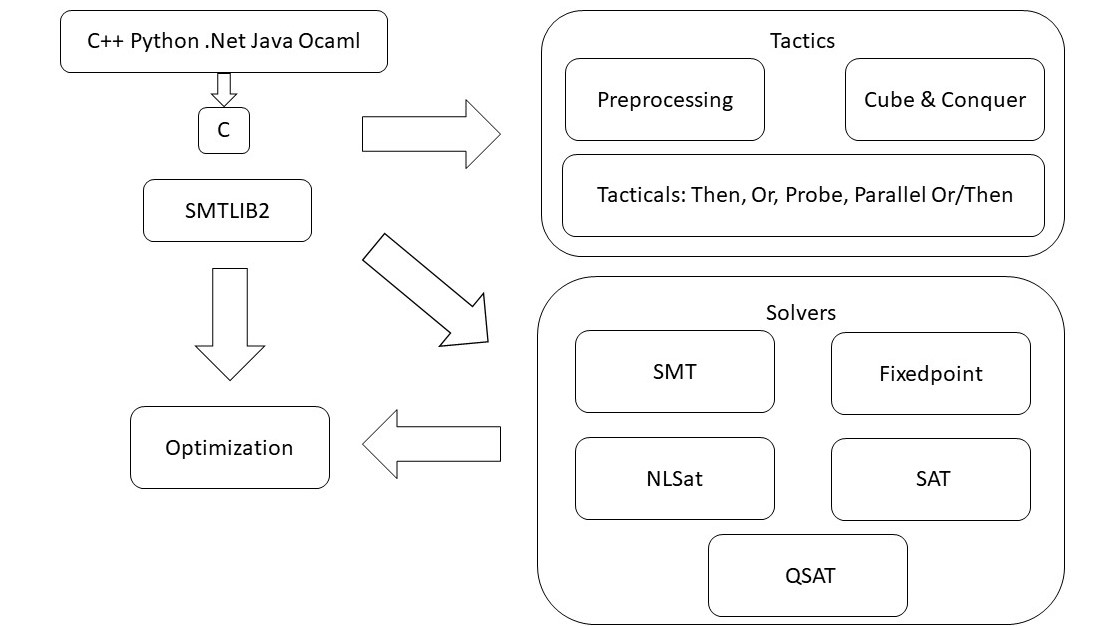
\includegraphics[width=.9\linewidth]{SMT}}%
    % fbox for "framed box"
  \end{center}
  \caption{%
     Overall system architecture of Z3
    \cite{nikolaj_bjorner_programming_nodate}
  }
  \label{fig:scholar} % NOTE: \label must appear after \caption
\end{figure}

Consider following example:
\begin{equation}
  \label{eq:example-sat}
  (Tie \lor Shirt) \land (\lnot Tie \lor Shirt) \land (\lnot Tie \lor \lnot Shirt)
\end{equation}

Formula \ref{eq:example-sat} can be solved in SMTLIB2 as following code:

\begin{figure}[ht]
  \begin{lstlisting} [language=SMTlIB2]
    (set-logic QF_UF)
    (declare-const Tie Bool)
    (declare-const Shirt Bool)
    (assert (or Tie Shirt))
    (assert (or (not Tie) Shirt))
    (assert (or (not Tie) (not Shirt)))
    (check-sat)
    (get-model)
  \end{lstlisting}
  \end{figure}

  This script will produce output of the code which is:


\begin{lstlisting} [language=SMTlIB2]
 sat
 (model
   (define-fun Tie () Bool false)
   (define-fun Shirt () Bool true)
 )
\end{lstlisting}
\vspace{1em}

This SMT-LIB2 script sets up the problem, declares the variables, asserts the constraints, checks for satisfiability,
  and retrieves the model, just like the Python code does with Z in the following example.

  Formula \ref{eq:example-sat} can also be solved by Z3 SMT solver as following code:

\begin{figure}[ht]
\begin{lstlisting}[language=Python]
  from z3 import Bools, Solver, Or, Not
  Tie, Shirt = Bools('Tie Shirt')
  s = Solver()
  s.add(Or(Tie, Shirt),
        Or(Not(Tie), Shirt),
        Or(Not(Tie), Not(Shirt)))
  print(s.check())
  print(s.model())
\end{lstlisting}
\end{figure}
The output of the code is:


\begin{lstlisting}[language=Python]
sat

[Tie = False, Shirt = True]
\end{lstlisting}

\begin{figure}[ht]
\begin{lstlisting}[language=Python]
  Z = IntSort()
  f = Function('f', Z, Z)
  x, y, z = Ints('x y z')
  A = Array('A', Z, Z)
  fml = Implies(x + 2 == y, f(Store(A, x, 3)[y - 2]) == f(y - x + 1))
  print(s.check(Not(fml)))
\end{lstlisting}
\end{figure}

\section{Working with LiquidHaskell}
\label{sec:lh}
LH is a tool that extends Haskell with refinement types. Refinement types are types that extend the expressiveness of Haskell types systems by providing predicates that can verify invarients of the program. In this section, we will explain how to use LH and how it works.
LH is available as a GHC plugin. To use LH, you need to add LH dependecy to the cabal file as following:

\vspace{1em}
\begin{lstlisting}
 cabal-version: 1.12

 name:           lh-plugin-demo
 version:        0.1.0.0
 ...
 ...
   build-depends:
       liquid-prelude,
       liquid-vector,
       liquidhaskell,
       base,
       containers,
       vector
   default-language: Haskell2010
   ghc-options:  -fplugin=LiquidHaskell
\end{lstlisting}
\vspace{1em}

By adding this dependency, LH can now check your program at compile time or via code linter in your IDE of choice. In following sections, we will explain how to use LH to verify the program.
\subsection{Type Refinement}
Refinement types allows to constrain the type of the variables by adding predicates to the types \cite{jhala_programming_2020}. For example we can define natural numbers as following:

\begin{haskell}
 {-@ type Nat = {v:Int | 0 <= v} @-}
\end{haskell}

Now if you configure your IDE to use Haskell LSP, it will show following error if you try to assign a negative number to a variable of type Nat.
\begin{haskell}
 {-@ x :: Nat @-}
 x = -1
 >>> typecheck: Liquid Type Mismatch
   .
   The inferred type
     VV : {v : GHC.Types.Int | v == GHC.Num.negate (GHC.Types.I# 1)
                               && v == (-GHC.Types.I# 1)}
   .
   is not a subtype of the required type
     VV : {VV##493 : GHC.Types.Int | VV##493 >= 0}
   .
   Constraint id 2
\end{haskell}
The error message shows that the inferred type of the variable x is not a subtype of the required type.

Using refinement types, one can define pre-conditions and post-conditions of the functions\cite{jhala_programming_2020}. 
For example, consider the following function:

\begin{haskell}
 tail :: [a] -> [a]
 tail (_:xs) = xs
 tail [] = error "tail: empty list"
\end{haskell}

The function defined above is a partial function because it does not handle the case when the list is empty. 
Typicall haskell types only allow to introduce the \textit{Maybe} type which postpone the handling of error to the other 
part of the program \cite{jhala_programming_2020}. Using refinement types, we can define the type of tail function as following:

\begin{haskell}
 {-@ tail :: {v:[a] | 0 < len v} -> a @-}
 tail :: [a] -> [a]
 tail (x:_) = x
\end{haskell}

Now our function is a total function as it doesn't allow non-empty list to be passed to \textit{tail}. However, it can't 
check the following case.

\begin{haskell}
 x :: [Int]
 x = tail (tail [1, 2])
\end{haskell}

When calling functions, LH won't look into the body of function to see if the first application of \textit{tail} gives the valid non-empty list to the second \textit{tail}.
To allow LH consider the above example as safe, we need to also specify post-condition for our function as following:

\begin{haskell}
 {-@ tail' :: xs: {v:[a] | 0 < len v} -> {v:[a] | len v == len xs - 1} @-}
 tail :: [a] -> [a]
 tail (x:_) = x
\end{haskell}
\subsection{Refined Data Types}
In the above examples, we saw how refinements of input and output of fucntion allows us to have stronger arguments about our program. 
We can take this further by refining the data types. Consider the following example:

\begin{haskell}
  data Slist a = Slist { size :: Int, elems :: [a] }

  {-@ data Slist a = Slist { size :: Nat, elems :: {v:[a] | len v == size} } @-}
\end{haskell}

In the above example, we introduced a new data type \textit{Slist} which is a list with a size. 
We also added a refinement to the data type that ensures that the size of the list is equal to the length of the list. 
This ensures that the size of the list is always correct.

The only thing in above example, that is missing is the definition of \textit{len}. Fortunately, this function has already reflected by
LH. In the following section, we show how can we use reflection or measure capabilities of LH to define and execute our own functions in the refinement logic and
reason about them.

\subsection{Lifting Functions to the Refinement Logic}
When our program become more complex, we need to define our own functions in the refinement logic and reason about
a function in another function. In LH, we can define our own functions in the refinement logic using reflection.
There are two ways to define a function in the refinement logic: reflection and measure. In this section, we will explain how to use reflection to define a function in the refinement logic.
\begin{haskell}

\end{haskell}

\begin{haskell}
 {-# OPTIONS_GHC -fplugin=LiquidHaskell #-}

 {-@ type Pos = {v:Int | 0 < v} @-}

 {-@ incr :: Pos -> Pos @-} //*\label{srcline:typerefinement}
 incr :: Int -> Int
 incr x = x + 1 
\end{haskell}

\subsection{Verification}

\section{Example Application}

In this section, we discuss the persistent stack data structure and how to verify its functional correctness using LiquidHaskell. Persistent data structures are immutable and support efficient access to previous versions. In this paper, we aim to prove the functional correctness of a persistent stack implementation, ensuring its operations satisfy the expected behavior.

\section{Definition of the Persistent Stack}
The stack is defined as a list-based data structure with two main operations: \texttt{push} and \texttt{pop}. Below is the Haskell implementation:

\begin{lstlisting}[caption=Persistent Stack Implementation]
{-@ LIQUID "--reflection" @-}
{-@ LIQUID "--ple" @-}

module PersistentStack where

-- Define the Stack type
data Stack a = Empty | Cons a (Stack a) deriving (Eq, Show)

-- Push operation
{-@ reflect push @-}
push :: a -> Stack a -> Stack a
push x s = Cons x s

-- Pop operation
{-@ reflect pop @-}
pop :: Stack a -> Maybe (a, Stack a)
pop Empty = Nothing
pop (Cons x s) = Just (x, s)

-- Top operation
{-@ reflect top @-}
top :: Stack a -> Maybe a
top Empty = Nothing
top (Cons x _) = Just x

-- IsEmpty operation
{-@ reflect isEmpty @-}
isEmpty :: Stack a -> Bool
isEmpty Empty = True
isEmpty _     = False
\end{lstlisting}

\section{Specification}
To prove the correctness of the \texttt{push} and \texttt{pop} operations, we define their specifications in LiquidHaskell.

\subsection{Push Operation}
The \texttt{push} operation adds an element to the stack. Its specification ensures that the new stack is not empty and that the top of the stack is the newly pushed element:

\begin{lstlisting}[caption=Push Specification]
{-@ pushSpec :: x:a -> s:Stack a 
  -> { top (push x s) == Just x && not (isEmpty (push x s)) } @-}
\end{lstlisting}

\subsection{Pop Operation}
The \texttt{pop} operation removes the top element from the stack. Its specification ensures that if the stack is non-empty, \texttt{pop} returns the correct element and the remainder of the stack:

\begin{lstlisting}[caption=Pop Specification]
{-@ popSpec :: s:Stack a -> { isEmpty s || case pop s of
    Nothing -> True;
    Just (x, s') -> top s == Just x && top (push x s') == Just x } @-}
\end{lstlisting}

\section{Proofs}
Using LiquidHaskell, we can prove the above specifications. Here, we outline the proof strategies for the main operations:

\subsection{Proof of Push Correctness}
The correctness of \texttt{push} follows directly from its definition:

\begin{align*}
\text{pushSpec:} \quad & \text{Let } s = \text{Empty or Cons.} \\
& \text{By definition of \texttt{push}, } \texttt{push x s} = \text{Cons } x s. \\
& \text{Then } \texttt{top (push x s)} = \text{Just } x. \\
& \text{Also, } \texttt{isEmpty (push x s)} = \text{False.}
\end{align*}

\subsection{Proof of Pop Correctness}
The correctness of \texttt{pop} depends on the case analysis of the stack:

\begin{itemize}
  \item Case \texttt{s = Empty}: \texttt{pop s = Nothing}, satisfying the specification.
  \item Case \texttt{s = Cons x s'}: \texttt{pop s = Just (x, s')}, ensuring \texttt{top s = Just x}.
\end{itemize}

\section{Conclusion}
This paper demonstrates the use of LiquidHaskell to verify the functional correctness of a persistent stack. Future work includes extending this methodology to more complex data structures such as queues and deques.
\label{sec:example}

\section{Conclusions, Results, Discussion}
\label{sec:conclusions}

%%%%%%%%%%%%%%%%%%%%%%%%%%%%%%%%%%%%%%%%%%%%%%%%%%%%%%%%%%%%%%%%%%%%%%%%%%%%%%%
\newpage
\nocite{*}
\bibliographystyle{eptcs}
\bibliography{references}

%%%%%%%%%%%%%%%%%%%%%%%%%%%%%%%%%%%%%%%%%%%%%%%%%%%%%%%%%%%%%%%%%%%%%%%%%%%%%%%
\end{document}
%%%%%%%%%%%%%%%%%%%%%%%%%%%%%%%%%%%%%%%%%%%%%%%%%%%%%%%%%%%%%%%%%%%%%%%%%%%%%%%
